\documentclass[aspectratio=169]{beamer}

% --- Toggle para version impresa (PDF) vs presentacion en vivo ---
% Cambiar \pptprinttrue por \pptprintfalse para version con animaciones embebidas
\newif\ifpptprint
\pptprinttrue

% --- Tema: solo colores, headline y footer custom ---
\usecolortheme{dolphin}
\setbeamertemplate{navigation symbols}{}
% --- Footline: condiciones de la figura (izq) + numero de diapositiva (der) ---
% Cada diapositiva con figura declara sus condiciones vía \cond{...}; el pie las
% imprime y las limpia, así la siguiente arranca vacía.
\gdef\condtext{}
\newcommand{\cond}[1]{\gdef\condtext{#1}}
\setbeamertemplate{footline}{%
  \vskip2pt
  {\color{gray!50}\hrule height 0.2pt}%
  \vskip3pt
  \hbox to\paperwidth{%
    \hskip1.2em
    % Alto fijo (3 renglones): si dependiera del texto, beamer calcularia mal
    % la altura util del cuerpo y las figuras se pasarian de la diapositiva.
    \begin{minipage}[t][19pt][t]{0.84\paperwidth}
      \raggedright\tiny\color{black!65}\condtext
    \end{minipage}%
    \hfill
    \begin{minipage}[t][19pt][t]{0.07\paperwidth}
      \raggedleft\tiny\color{black!65}\insertframenumber\,/\,\inserttotalframenumber
    \end{minipage}%
    \hskip1.2em}%
  \vskip4pt
  \gdef\condtext{}%
}

% --- Paquetes ---
\usepackage[utf8]{inputenc}
\usepackage[T1]{fontenc}
\usepackage[spanish,es-nodecimaldot]{babel}
\usepackage{amsmath,amssymb}
\usepackage{graphicx}
\usepackage{booktabs}
\usepackage{tikz}
\usepackage{hyperref}

% ============================================================
% Headline: grupos de puntos por seccion / estudio
% ============================================================
% Un punto por diapositiva. Los rangos de abajo deben coincidir con los
% numeros de frame reales: si se agregan o quitan diapositivas hay que
% actualizar los pares (primero,ultimo) de cada \dgrp.
\newcommand{\dgrp}[3]{% #1 = primer frame, #2 = ultimo frame, #3 = etiqueta
  \pgfmathtruncatemacro{\nd}{#2-#1+1}%
  \foreach \fr [count=\k from 0] in {#1,...,#2} {%
    \pgfmathsetmacro{\x}{\bx + \k*\dgap}%
    \ifnum\fr=\cf
      \fill[white] (\x,0) circle(\rad);
      \draw[white,line width=0.8pt] (\x,0) circle(\rad+1.2pt);
    \else\ifnum\fr<\cf
      \fill[white] (\x,0) circle(\rad);
    \else
      \draw[white,line width=0.4pt] (\x,0) circle(\rad);
    \fi\fi
  }%
  \node[white,font=\tiny\bfseries]
    at ({\bx+(\nd-1)*\dgap/2},-0.34) {#3};%
  \pgfmathsetmacro{\bxtmp}{\bx + (\nd-1)*\dgap + \sgap}%
  \let\bx\bxtmp
}

\setbeamertemplate{headline}{%
  \begin{beamercolorbox}[ht=2.9em,dp=0.1em,leftskip=0pt,rightskip=0pt]{section in head/foot}%
    \centering
    \begin{tikzpicture}
      \pgfmathtruncatemacro{\cf}{\insertframenumber}
      \def\rad{1.5pt}
      \def\dgap{0.19}
      \def\sgap{0.55}
      \pgfmathsetmacro{\bx}{0}

      \dgrp{3}{5}{Intro}
      \dgrp{6}{8}{Impl}
      \dgrp{9}{12}{Sim}
      \dgrp{13}{28}{b}
      \dgrp{29}{38}{c}
      \dgrp{39}{48}{d}
      \dgrp{49}{53}{e}
      \dgrp{54}{55}{CIM}
      \dgrp{56}{58}{Conc}
    \end{tikzpicture}
  \end{beamercolorbox}
}

% ============================================================
% Comandos de notacion y de armado de diapositivas
% ============================================================
\newcommand{\vv}[1]{\boldsymbol{#1}}   % vectores en negrita
\newcommand{\uu}[1]{\mathrm{#1}}       % unidades en romano

% Diapositiva separadora de seccion (solo el titulo, sin numerar la seccion)
\newcommand{\seccion}[1]{%
  \begin{frame}
    \vfill
    \begin{center}{\Huge\bfseries #1}\end{center}
    \vfill
  \end{frame}
}

% Parametros fijos, comunes a todas las figuras (van al pie, no dentro)
\newcommand{\pfijos}{%
  $L = 1\times10^{1}\;\uu{m}$, contornos periodicos;
  $r_c = 1\;\uu{m}$;
  $v = 3\times10^{-2}\;\uu{m/s}$;
  $\Delta t = 1\;\uu{s}$;
  $3\times10^{4}$ pasos;
  1 corrida (semilla fija)%
}

% Figura unica, al maximo tamano posible. Las condiciones van al pie.
\newcommand{\figuno}[2]{% #1 = imagen, #2 = condiciones
  \cond{#2}%
  \begin{center}
    \includegraphics[width=\textwidth,height=0.80\textheight,keepaspectratio]{#1}
  \end{center}
}

% Dos figuras lado a lado (comparacion), cada una con su titulo justo debajo.
% El par se centra en \paperwidth (no en \textwidth) para ganar ancho: el \hss
% de los costados absorbe el desborde sin que LaTeX avise por overfull.
\newcommand{\figdos}[5]{% #1 = izq, #2 = titulo izq, #3 = der, #4 = titulo der, #5 = condiciones
  \cond{#5}%
  \begin{center}
    \hbox to \textwidth{\hss
      \begin{minipage}[t]{0.48\paperwidth}
        \centering
        \includegraphics[width=\linewidth,height=0.74\textheight,keepaspectratio]{#1}
        \par\vspace{0.5em}{\small #2}
      \end{minipage}%
      \hspace{0.015\paperwidth}%
      \begin{minipage}[t]{0.48\paperwidth}
        \centering
        \includegraphics[width=\linewidth,height=0.74\textheight,keepaspectratio]{#3}
        \par\vspace{0.5em}{\small #4}
      \end{minipage}%
    \hss}
  \end{center}
}

% Placeholder de animacion.
% Version impresa (PDF de entrega): fotograma fijo + link explicito debajo.
% Version en vivo: animacion embebida en la diapositiva.
\newcommand{\animph}[2]{% #1 = condiciones, #2 = link
  \cond{#1}%
  \begin{center}
  \ifpptprint
    \begin{tikzpicture}
      \draw[dashed,gray,line width=1pt] (0,0) rectangle (13.4,4.4);
      \node[gray,font=\normalsize] at (6.7,2.6)
        {[Fotograma representativo de la animacion]};
      \node[gray,font=\small] at (6.7,1.9)
        {reemplazar por la captura correspondiente};
    \end{tikzpicture}
    \par\vspace{0.5em}
    {\footnotesize Video: \href{#2}{\texttt{#2}}}
  \else
    \begin{tikzpicture}
      \draw[dashed,gray,line width=1pt] (0,0) rectangle (13.4,5.0);
      \node[gray,font=\normalsize] at (6.7,2.5) {[Animacion embebida]};
    \end{tikzpicture}
  \fi
  \end{center}
}

% --- Metadatos ---
\title{Automatas Celulares Off-Lattice}
\subtitle{Simulacion de bandadas de agentes autopropulsados}
\author{Miembro 1 \and Miembro 2 \and Miembro 3}
\institute{Simulacion de Sistemas --- ITBA}
\date{Septiembre 2026}

% ============================================================
\begin{document}

% --- Frame 1: Titulo ---
\begin{frame}
  \titlepage
\end{frame}

% --- Frame 2: Indice ---
\begin{frame}{Contenidos}
  \tableofcontents
\end{frame}

% ============================================================
\section{Introduccion / Sistema Real}
% Frames 3-5
% ============================================================

% --- Frame 3 ---
\seccion{Introduccion / Sistema Real}

% --- Frame 4 ---
\begin{frame}{Introduccion}
  \begin{itemize}
    \item Sistema de particulas autopropulsadas con interaccion local
    \item Transicion de fase: desorden $\leftrightarrow$ flocking
      segun el ruido $\eta$
    \item Dos reglas de interaccion: Vicsek (promedio) y Votante (copia)
  \end{itemize}
\end{frame}

% --- Frame 5 ---
\begin{frame}{Modelo Matematico}
  \begin{columns}[T]
    \column{0.55\textwidth}
    \textbf{Estandar (Vicsek):}
    \[
      \bar{\theta}_i = \operatorname{atan2}\!\Big(
        \sum_{j \in \mathcal{N}_i} \sin\theta_j,\;
        \sum_{j \in \mathcal{N}_i} \cos\theta_j \Big)
    \]
    \vspace{0.3em}
    \footnotesize
    $\mathcal{N}_i$ incluye a la particula $i$ y sus vecinos
    dentro de $r_c$.

    \column{0.4\textwidth}
    \textbf{Votante:}
    \[
      \bar{\theta}_i = \theta_j, \quad j \in \mathcal{N}_i
    \]
    \vspace{0.5em}
    \small
    Copia la direccion de un vecino al azar.

    \vspace{1em}
    \textbf{Ambos modelos:}
    \[
      \theta_i(t\!+\!1) = \bar{\theta}_i + \eta\,\xi
    \]
    \[
      \vv{r}_i(t\!+\!1) = \vv{r}_i(t) + v\,
      \begin{pmatrix}\cos\theta_i(t\!+\!1) \\
                     \sin\theta_i(t\!+\!1)\end{pmatrix}
    \]
    \footnotesize
    $\xi \sim \mathcal{U}[-1/2,\,1/2]$,
    contornos periodicos.
  \end{columns}
\end{frame}

% ============================================================
\section{Implementacion}
% Frames 6-8
% ============================================================

% --- Frame 6 ---
\seccion{Implementacion}

% --- Frame 7 ---
\begin{frame}{Arquitectura del codigo}
  \begin{center}
    \begin{tikzpicture}[
        box/.style={draw, rounded corners, minimum width=3cm,
                     minimum height=0.75cm, font=\small},
        arr/.style={->, thick}
      ]
      \node[box] (cfg) at (0,3.0) {main.cpp};
      \node[box] (eng) at (0,1.8) {SimulationEngine};
      \node[box] (cim) at (0,0.6) {CellIndexMethod};
      \node[box] (out) at (0,-0.6) {OutputWriter};

      \draw[arr] (cfg) -- (eng);
      \draw[arr] (eng) -- (cim);
      \draw[arr] (eng) -- (out);

      \node[right, font=\footnotesize, text=gray] at (1.7,3.0) {args, semilla};
      \node[right, font=\footnotesize, text=gray] at (1.7,1.8) {paso, observables};
      \node[right, font=\footnotesize, text=gray] at (1.7,0.6) {vecinos};
      \node[right, font=\footnotesize, text=gray] at (1.7,-0.6) {estado del sistema};
    \end{tikzpicture}
  \end{center}
\end{frame}

% --- Frame 8 ---
\begin{frame}{Metodo del Indice Celular (CIM)}
  \begin{itemize}
    \item Grilla $M \times M$, celdas de tamano $\geq r_c$
    \item Listas enlazadas con arreglos planos (cache-friendly)
    \item Solo se inspeccionan 9 celdas vecinas
      $\Rightarrow$ busqueda en $\mathcal{O}(N)$
    \item Contornos periodicos con envoltura modular
  \end{itemize}
\end{frame}

% ============================================================
\section{Simulaciones}
% Frames 9-12
% ============================================================

% --- Frame 9 ---
\seccion{Simulaciones}

% --- Frame 10 ---
\begin{frame}{Geometria del sistema}
  \begin{columns}[T]
    \column{0.5\textwidth}
    \begin{itemize}
      \item Caja cuadrada $L \times L$, $L = 1\times10^{1}\;\uu{m}$
      \item Contornos periodicos (topologia toroidal)
      \item Radio de interaccion $r_c = 1\;\uu{m}$
      \item Velocidad constante $v = 3\times10^{-2}\;\uu{m/s}$
      \item Paso temporal $\Delta t = 1\;\uu{s}$
    \end{itemize}

    \column{0.45\textwidth}
    \begin{center}
    \begin{tikzpicture}[scale=1.2]
      \draw[thick] (0,0) rectangle (4,4);
      \foreach \x/\y/\a in {0.8/2.1/30, 2.2/3.5/120, 1.5/0.8/200,
                             3.1/2.7/80, 0.5/3.2/310, 3.6/1.0/170} {
        \draw[->, thick, blue!70!black]
          (\x,\y) -- ++({cos(\a)*0.35},{sin(\a)*0.35});
        \fill[blue!40] (\x,\y) circle (2pt);
      }
      \node[below] at (2,-0.15) {\small $L$};
      \node[left]  at (-0.15,2) {\rotatebox{90}{\small $L$}};
    \end{tikzpicture}
    \end{center}
  \end{columns}
\end{frame}

% --- Frame 11 ---
\begin{frame}{Observables}
  \begin{columns}[T]
    \column{0.5\textwidth}
    \textbf{Polarizacion}
    \[
      v_a(t) = \left|
        \frac{1}{N} \sum_{i=1}^{N}
        \begin{pmatrix}
          \cos\theta_i(t) \\
          \sin\theta_i(t)
        \end{pmatrix}
      \right|
    \]
    \small
    Grado de alineacion global.\\
    $v_a = 1$: totalmente alineado.\\
    $v_a \approx 0$: desordenado.

    \column{0.5\textwidth}
    \textbf{Fraccion del cluster mas grande}
    \[
      S(t) = \frac{N_{\text{cluster}}}{N}
    \]
    \small
    Un cluster es un conjunto de particulas donde todo par
    esta conectado por una cadena de vecinos dentro de $r_c$.
    Se calcula con BFS sobre el grafo de vecindad.
  \end{columns}

  \vspace{0.6em}
  \footnotesize
  \textbf{Escalar caracteristico:} promedio temporal de cada observable
  entre $t_{\text{ini}}$ (inicio del estacionario) y $3\times10^{4}$ pasos;
  la barra de error es el desvio de esa serie en el estacionario.
\end{frame}

% --- Frame 12 ---
\begin{frame}{Parametros del estudio}
  \begin{table}
    \centering\small
    \begin{tabular}{@{}lll@{}}
      \toprule
      Parametro & Valores & Descripcion \\
      \midrule
      $\eta$ (Estandar) & $0;\,0.25;\,\ldots;\,5$ & 21 valores \\
      $\eta$ (Votante) & $0;\,0.05;\,\ldots;\,1$ & 21 valores \\
      $\rho$ (densidad) & $2;\,4;\,8\;\uu{m^{-2}}$ & Pedidas por el enunciado \\
      $\rho$ (baja) & $1/\pi;\,1/2\pi;\,1/3\pi\;\uu{m^{-2}}$ & Regimen diluido \\
      $N = \rho L^2$ & $1\times10^{1}$ a $8\times10^{2}$ & Particulas \\
      $L$ & $1\times10^{1}\;\uu{m}$ & Fijo \\
      $r_c$ & $1\;\uu{m}$ & Fijo \\
      $v$ & $3\times10^{-2}\;\uu{m/s}$ & Fijo \\
      Pasos & $3\times10^{4}$ & Por corrida \\
      Repeticiones & $1$ & Semilla fija \\
      \bottomrule
    \end{tabular}
  \end{table}
  \vspace{0.2em}
  \footnotesize
  Con una sola realizacion, la barra de error es la fluctuacion temporal
  del observable dentro del estacionario.
\end{frame}

% ============================================================
\section{Resultados}
% Frames 13-53
% ============================================================

% --- Frame 13 ---
\seccion{Resultados}

% ------------------------------------------------------------
% b) Evolucion temporal de la polarizacion   (frames 14-28)
% ------------------------------------------------------------

% ---- rho = 2 ----

% --- Frame 14 ---
\begin{frame}{Animacion --- Estandar, $\rho = 2\;\uu{m^{-2}}$}
  \animph{\pfijos. \textbf{Estandar}; $\rho = 2\;\uu{m^{-2}}$, $N = 2\times10^{2}$; $\eta = 0.5$ y $\eta = 3.5$.}{https://youtu.be/XXXXX}
\end{frame}

% --- Frame 15 ---
\begin{frame}{Evolucion de la polarizacion --- Estandar, $\rho = 2\;\uu{m^{-2}}$}
  \figuno{entrega/b/evolucion_va_ruidos_30000_rho2.png}{\pfijos. \textbf{Estandar}; $\rho = 2\;\uu{m^{-2}}$, $N = 2\times10^{2}$; $\eta = 0.5;\ 1.5;\ 3.5$. Lineas verticales: inicio del estacionario ($t_{\text{ini}}$).}
\end{frame}

% --- Frame 16 ---
\begin{frame}{Animacion --- Votante, $\rho = 2\;\uu{m^{-2}}$}
  \animph{\pfijos. \textbf{Votante}; $\rho = 2\;\uu{m^{-2}}$, $N = 2\times10^{2}$; $\eta = 0.05$ y $\eta = 0.5$.}{https://youtu.be/XXXXX}
\end{frame}

% --- Frame 17 ---
\begin{frame}{Evolucion de la polarizacion --- Votante, $\rho = 2\;\uu{m^{-2}}$}
  \figuno{entrega/b/evolucion_va_voter_30000_rho2.png}{\pfijos. \textbf{Votante}; $\rho = 2\;\uu{m^{-2}}$, $N = 2\times10^{2}$; $\eta = 0.05;\ 0.5$. Lineas verticales: inicio del estacionario ($t_{\text{ini}}$).}
\end{frame}

% --- Frame 18 ---
\begin{frame}{Comparacion Estandar vs Votante --- $v_a(t)$, $\rho = 2\;\uu{m^{-2}}$}
  \figdos%
    {entrega/b/evolucion_va_ruidos_30000_rho2.png}%
    {Estandar}%
    {entrega/b/evolucion_va_voter_30000_rho2.png}%
    {Votante}%
    {\pfijos. $\rho = 2\;\uu{m^{-2}}$; $N = 2\times10^{2}$.}
\end{frame}

% ---- rho = 4 ----

% --- Frame 19 ---
\begin{frame}{Animacion --- Estandar, $\rho = 4\;\uu{m^{-2}}$}
  \animph{\pfijos. \textbf{Estandar}; $\rho = 4\;\uu{m^{-2}}$, $N = 4\times10^{2}$; $\eta = 0.5$ y $\eta = 3.5$.}{https://youtu.be/XXXXX}
\end{frame}

% --- Frame 20 ---
\begin{frame}{Evolucion de la polarizacion --- Estandar, $\rho = 4\;\uu{m^{-2}}$}
  \figuno{entrega/b/evolucion_va_ruidos_30000.png}{\pfijos. \textbf{Estandar}; $\rho = 4\;\uu{m^{-2}}$, $N = 4\times10^{2}$; $\eta = 0.5;\ 1.5;\ 3.5$. Lineas verticales: inicio del estacionario ($t_{\text{ini}}$).}
\end{frame}

% --- Frame 21 ---
\begin{frame}{Animacion --- Votante, $\rho = 4\;\uu{m^{-2}}$}
  \animph{\pfijos. \textbf{Votante}; $\rho = 4\;\uu{m^{-2}}$, $N = 4\times10^{2}$; $\eta = 0.05$ y $\eta = 0.5$.}{https://youtu.be/XXXXX}
\end{frame}

% --- Frame 22 ---
\begin{frame}{Evolucion de la polarizacion --- Votante, $\rho = 4\;\uu{m^{-2}}$}
  \figuno{entrega/b/evolucion_va_voter_30000.png}{\pfijos. \textbf{Votante}; $\rho = 4\;\uu{m^{-2}}$, $N = 4\times10^{2}$; $\eta = 0.05;\ 0.5$. Lineas verticales: inicio del estacionario ($t_{\text{ini}}$).}
\end{frame}

% --- Frame 23 ---
\begin{frame}{Comparacion Estandar vs Votante --- $v_a(t)$, $\rho = 4\;\uu{m^{-2}}$}
  \figdos%
    {entrega/b/evolucion_va_ruidos_30000.png}%
    {Estandar}%
    {entrega/b/evolucion_va_voter_30000.png}%
    {Votante}%
    {\pfijos. $\rho = 4\;\uu{m^{-2}}$; $N = 4\times10^{2}$.}
\end{frame}

% ---- rho = 8 ----

% --- Frame 24 ---
\begin{frame}{Animacion --- Estandar, $\rho = 8\;\uu{m^{-2}}$}
  \animph{\pfijos. \textbf{Estandar}; $\rho = 8\;\uu{m^{-2}}$, $N = 8\times10^{2}$; $\eta = 0.5$ y $\eta = 3.5$.}{https://youtu.be/XXXXX}
\end{frame}

% --- Frame 25 ---
\begin{frame}{Evolucion de la polarizacion --- Estandar, $\rho = 8\;\uu{m^{-2}}$}
  \figuno{entrega/b/evolucion_va_ruidos_30000_rho8.png}{\pfijos. \textbf{Estandar}; $\rho = 8\;\uu{m^{-2}}$, $N = 8\times10^{2}$; $\eta = 0.5;\ 1.5;\ 3.5$. Lineas verticales: inicio del estacionario ($t_{\text{ini}}$).}
\end{frame}

% --- Frame 26 ---
\begin{frame}{Animacion --- Votante, $\rho = 8\;\uu{m^{-2}}$}
  \animph{\pfijos. \textbf{Votante}; $\rho = 8\;\uu{m^{-2}}$, $N = 8\times10^{2}$; $\eta = 0.05$ y $\eta = 0.5$.}{https://youtu.be/XXXXX}
\end{frame}

% --- Frame 27 ---
\begin{frame}{Evolucion de la polarizacion --- Votante, $\rho = 8\;\uu{m^{-2}}$}
  \figuno{entrega/b/evolucion_va_voter_30000_rho8.png}{\pfijos. \textbf{Votante}; $\rho = 8\;\uu{m^{-2}}$, $N = 8\times10^{2}$; $\eta = 0.05;\ 0.5$. Lineas verticales: inicio del estacionario ($t_{\text{ini}}$).}
\end{frame}

% --- Frame 28 ---
\begin{frame}{Comparacion Estandar vs Votante --- $v_a(t)$, $\rho = 8\;\uu{m^{-2}}$}
  \figdos%
    {entrega/b/evolucion_va_ruidos_30000_rho8.png}%
    {Estandar}%
    {entrega/b/evolucion_va_voter_30000_rho8.png}%
    {Votante}%
    {\pfijos. $\rho = 8\;\uu{m^{-2}}$; $N = 8\times10^{2}$.}
\end{frame}

% ------------------------------------------------------------
% c) Polarizacion media vs ruido   (frames 29-38)
% ------------------------------------------------------------

% ---- densidades 2, 4, 8 ----

% --- Frame 29 ---
\begin{frame}{Animacion --- Estandar, barrido de $\eta$}
  \animph{\pfijos. \textbf{Estandar}; $\rho = 2;\ 4;\ 8\;\uu{m^{-2}}$; Extremos del barrido:; $\eta = 0$ y $\eta = 5$.}{https://youtu.be/XXXXX}
\end{frame}

% --- Frame 30 ---
\begin{frame}{$\langle v_a \rangle$ vs $\eta$ --- Estandar}
  \figuno{entrega/c/c_standard_3dens_30000.png}{\pfijos. \textbf{Estandar}; $\rho = 2;\ 4;\ 8\;\uu{m^{-2}}$; $N = 2;\,4;\,8 \times10^{2}$; $\eta = 0$ a $5$, paso $0.25$. Promedio y desvio en el estacionario.}
\end{frame}

% --- Frame 31 ---
\begin{frame}{Animacion --- Votante, barrido de $\eta$}
  \animph{\pfijos. \textbf{Votante}; $\rho = 2;\ 4;\ 8\;\uu{m^{-2}}$; Extremos del barrido:; $\eta = 0$ y $\eta = 1$.}{https://youtu.be/XXXXX}
\end{frame}

% --- Frame 32 ---
\begin{frame}{$\langle v_a \rangle$ vs $\eta$ --- Votante}
  \figuno{entrega/c/c_voter_3dens_30000.png}{\pfijos. \textbf{Votante}; $\rho = 2;\ 4;\ 8\;\uu{m^{-2}}$; $N = 2;\,4;\,8 \times10^{2}$; $\eta = 0$ a $1$, paso $0.05$. Promedio y desvio en el estacionario.}
\end{frame}

% --- Frame 33 ---
\begin{frame}{Comparacion Estandar vs Votante --- $\langle v_a \rangle$ vs $\eta$}
  \figdos%
    {entrega/c/c_standard_3dens_30000.png}%
    {Estandar ($\eta \leq 5$)}%
    {entrega/c/c_voter_3dens_30000.png}%
    {Votante ($\eta \leq 1$)}%
    {\pfijos. $\rho = 2;\ 4;\ 8\;\uu{m^{-2}}$. Notar la diferencia de escala en $\eta$.}
\end{frame}

% ---- densidades bajas ----

% --- Frame 34 ---
\begin{frame}{Animacion --- Estandar, densidades bajas}
  \animph{\pfijos. \textbf{Estandar}; $\rho = 1/\pi;\ 1/2\pi;\ 1/3\pi\;\uu{m^{-2}}$; $N = 31;\ 15;\ 10$; $\eta = 0$ y $\eta = 5$.}{https://youtu.be/XXXXX}
\end{frame}

% --- Frame 35 ---
\begin{frame}{$\langle v_a \rangle$ vs $\eta$ --- Estandar, densidades bajas}
  \figuno{entrega/c/c_standard_lowdens_30000.png}{\pfijos. \textbf{Estandar}; $\rho = 1/\pi;\ 1/2\pi;\ 1/3\pi\;\uu{m^{-2}}$; $N = 31;\ 15;\ 10$; $\eta = 0$ a $5$, paso $0.25$.}
\end{frame}

% --- Frame 36 ---
\begin{frame}{Animacion --- Votante, densidades bajas}
  \animph{\pfijos. \textbf{Votante}; $\rho = 1/\pi;\ 1/3\pi\;\uu{m^{-2}}$; $N = 31;\ 10$; $\eta = 0$ y $\eta = 1$.}{https://youtu.be/XXXXX}
\end{frame}

% --- Frame 37 ---
\begin{frame}{$\langle v_a \rangle$ vs $\eta$ --- Votante, densidades bajas}
  \figuno{entrega/c/c_voter_lowdens_30000.png}{\pfijos. \textbf{Votante}; $\rho = 1/\pi;\ 1/3\pi\;\uu{m^{-2}}$; $N = 31;\ 10$; $\eta = 0$ a $1$, paso $0.05$.}
\end{frame}

% --- Frame 38 ---
\begin{frame}{Comparacion --- $\langle v_a \rangle$ vs $\eta$, densidades bajas}
  \figdos%
    {entrega/c/c_standard_lowdens_30000.png}%
    {Estandar}%
    {entrega/c/c_voter_lowdens_30000.png}%
    {Votante}%
    {\pfijos. Regimen diluido; $\rho \leq 1/\pi\;\uu{m^{-2}}$.}
\end{frame}

% ------------------------------------------------------------
% d) Cluster mas grande   (frames 39-48)
% ------------------------------------------------------------

% ---- d-1) evolucion de S(t) ----

% --- Frame 39 ---
\begin{frame}{Animacion --- Estandar, clusters}
  \animph{\pfijos. \textbf{Estandar}; $\rho = 2\;\uu{m^{-2}}$ ($N = 2\times10^{2}$); vs $\rho = 1/\pi\;\uu{m^{-2}}$ ($N = 31$); $\eta = 0.5$.}{https://youtu.be/XXXXX}
\end{frame}

% --- Frame 40 ---
\begin{frame}{Evolucion de $S$ --- Estandar}
  \figuno{entrega/d1/d1_standard_2_vs_low_30000.png}{\pfijos. \textbf{Estandar}; $\rho = 2$ y $1/\pi\;\uu{m^{-2}}$; $N = 2\times10^{2}$ y $31$; $\eta = 0.5$. Lineas verticales: inicio del estacionario ($t_{\text{ini}}$).}
\end{frame}

% --- Frame 41 ---
\begin{frame}{Animacion --- Votante, clusters}
  \animph{\pfijos. \textbf{Votante}; $\rho = 2\;\uu{m^{-2}}$ ($N = 2\times10^{2}$); vs $\rho = 1/\pi\;\uu{m^{-2}}$ ($N = 31$); $\eta = 0.1$.}{https://youtu.be/XXXXX}
\end{frame}

% --- Frame 42 ---
\begin{frame}{Evolucion de $S$ --- Votante}
  \figuno{entrega/d1/d1_voter_2_vs_low_30000.png}{\pfijos. \textbf{Votante}; $\rho = 2$ y $1/\pi\;\uu{m^{-2}}$; $N = 2\times10^{2}$ y $31$; $\eta = 0.1$. Lineas verticales: inicio del estacionario ($t_{\text{ini}}$).}
\end{frame}

% --- Frame 43 ---
\begin{frame}{Comparacion Estandar vs Votante --- $S(t)$}
  \figdos%
    {entrega/d1/d1_standard_2_vs_low_30000.png}%
    {Estandar ($\eta = 0.5$)}%
    {entrega/d1/d1_voter_2_vs_low_30000.png}%
    {Votante ($\eta = 0.1$)}%
    {\pfijos. $\rho = 2$ y $1/\pi\;\uu{m^{-2}}$.}
\end{frame}

% ---- d-2) <S> vs eta ----

% --- Frame 44 ---
\begin{frame}{Animacion --- Estandar, barrido de $\eta$ (clusters)}
  \animph{\pfijos. \textbf{Estandar}; $\rho = 2$ y $1/\pi\;\uu{m^{-2}}$; Extremos del barrido:; $\eta = 0$ y $\eta = 5$.}{https://youtu.be/XXXXX}
\end{frame}

% --- Frame 45 ---
\begin{frame}{$\langle S \rangle$ vs $\eta$ --- Estandar}
  \figuno{entrega/d2/d2_standard_2_vs_low_30000.png}{\pfijos. \textbf{Estandar}; $\rho = 2$ y $1/\pi\;\uu{m^{-2}}$; $N = 2\times10^{2}$ y $31$; $\eta = 0$ a $5$, paso $0.25$. Promedio y desvio en el estacionario.}
\end{frame}

% --- Frame 46 ---
\begin{frame}{Animacion --- Votante, barrido de $\eta$ (clusters)}
  \animph{\pfijos. \textbf{Votante}; $\rho = 2$ y $1/\pi\;\uu{m^{-2}}$; Extremos del barrido:; $\eta = 0$ y $\eta = 1$.}{https://youtu.be/XXXXX}
\end{frame}

% --- Frame 47 ---
\begin{frame}{$\langle S \rangle$ vs $\eta$ --- Votante}
  \figuno{entrega/d2/d2_voter_2_vs_low_30000.png}{\pfijos. \textbf{Votante}; $\rho = 2$ y $1/\pi\;\uu{m^{-2}}$; $N = 2\times10^{2}$ y $31$; $\eta = 0$ a $1$, paso $0.05$. Promedio y desvio en el estacionario.}
\end{frame}

% --- Frame 48 ---
\begin{frame}{Comparacion Estandar vs Votante --- $\langle S \rangle$ vs $\eta$}
  \figdos%
    {entrega/d2/d2_standard_2_vs_low_30000.png}%
    {Estandar ($\eta \leq 5$)}%
    {entrega/d2/d2_voter_2_vs_low_30000.png}%
    {Votante ($\eta \leq 1$)}%
    {\pfijos. $\rho = 2$ y $1/\pi\;\uu{m^{-2}}$. Notar la diferencia de escala en $\eta$.}
\end{frame}

% ------------------------------------------------------------
% e) Polarizacion vs componente gigante   (frames 49-53)
% ------------------------------------------------------------

% --- Frame 49 ---
\begin{frame}{Animacion --- Estandar, $v_a$ vs $S$}
  \animph{\pfijos. \textbf{Estandar}; $\rho = 1/3\pi;\ 1/\pi;\ 2;\ 8\;\uu{m^{-2}}$; Extremos: $\eta = 0$ y $\eta = 5$.}{https://youtu.be/XXXXX}
\end{frame}

% --- Frame 50 ---
\begin{frame}{$\langle v_a \rangle$ vs $\langle S \rangle$ --- Estandar}
  \figuno{entrega/e/e_standard_4dens_30000.png}{\pfijos. \textbf{Estandar}; $\rho = 1/3\pi;\ 1/\pi;\ 2;\ 8\;\uu{m^{-2}}$; $N = 10;\ 31;\ 2\times10^{2};\ 8\times10^{2}$; $\eta = 0;\,0.5;\,1;\,1.5;\,2;\,2.5;\,3;\,4;\,5$.}
\end{frame}

% --- Frame 51 ---
\begin{frame}{Animacion --- Votante, $v_a$ vs $S$}
  \animph{\pfijos. \textbf{Votante}; $\rho = 1/3\pi;\ 1/\pi;\ 2;\ 8\;\uu{m^{-2}}$; Extremos: $\eta = 0.05$ y $\eta = 1$.}{https://youtu.be/XXXXX}
\end{frame}

% --- Frame 52 ---
\begin{frame}{$\langle v_a \rangle$ vs $\langle S \rangle$ --- Votante}
  \figuno{entrega/e/e_voter_4dens_30000.png}{\pfijos. \textbf{Votante}; $\rho = 1/3\pi;\ 1/\pi;\ 2;\ 8\;\uu{m^{-2}}$; $N = 10;\ 31;\ 2\times10^{2};\ 8\times10^{2}$; $\eta = 0.05;\,0.1;\,0.2;\,0.4;\,0.6;\,0.8;\,1$.}
\end{frame}

% --- Frame 53 ---
\begin{frame}{Comparacion Estandar vs Votante --- $\langle v_a \rangle$ vs $\langle S \rangle$}
  \figdos%
    {entrega/e/e_standard_4dens_30000.png}%
    {Estandar}%
    {entrega/e/e_voter_4dens_30000.png}%
    {Votante}%
    {\pfijos. $\rho = 1/3\pi;\ 1/\pi;\ 2;\ 8\;\uu{m^{-2}}$.}
\end{frame}

% ============================================================
\section{Desempeno (CIM)}
% Frames 54-55
% ============================================================

% --- Frame 54 ---
\seccion{Desempeno del CIM}

% --- Frame 55 ---
\begin{frame}{Tiempos de ejecucion del CIM --- comparacion con TP1}
  \cond{Mismo kernel en ambas series, solo cambia la geometria:
    \textbf{TP1} $L = 2\times10^{1}\;\uu{m}$, $M = 13$;
    \textbf{TP2} $L = 1\times10^{1}\;\uu{m}$, $M = 10$.
    $r_c = 1\;\uu{m}$, contornos periodicos; configuracion estatica (sin evolucionar
    la simulacion); lotes de $1\times10^{2}$ corridas; $N = 10$ a $1\times10^{3}$;
    media y desvio sobre las muestras.}
  \begin{center}
    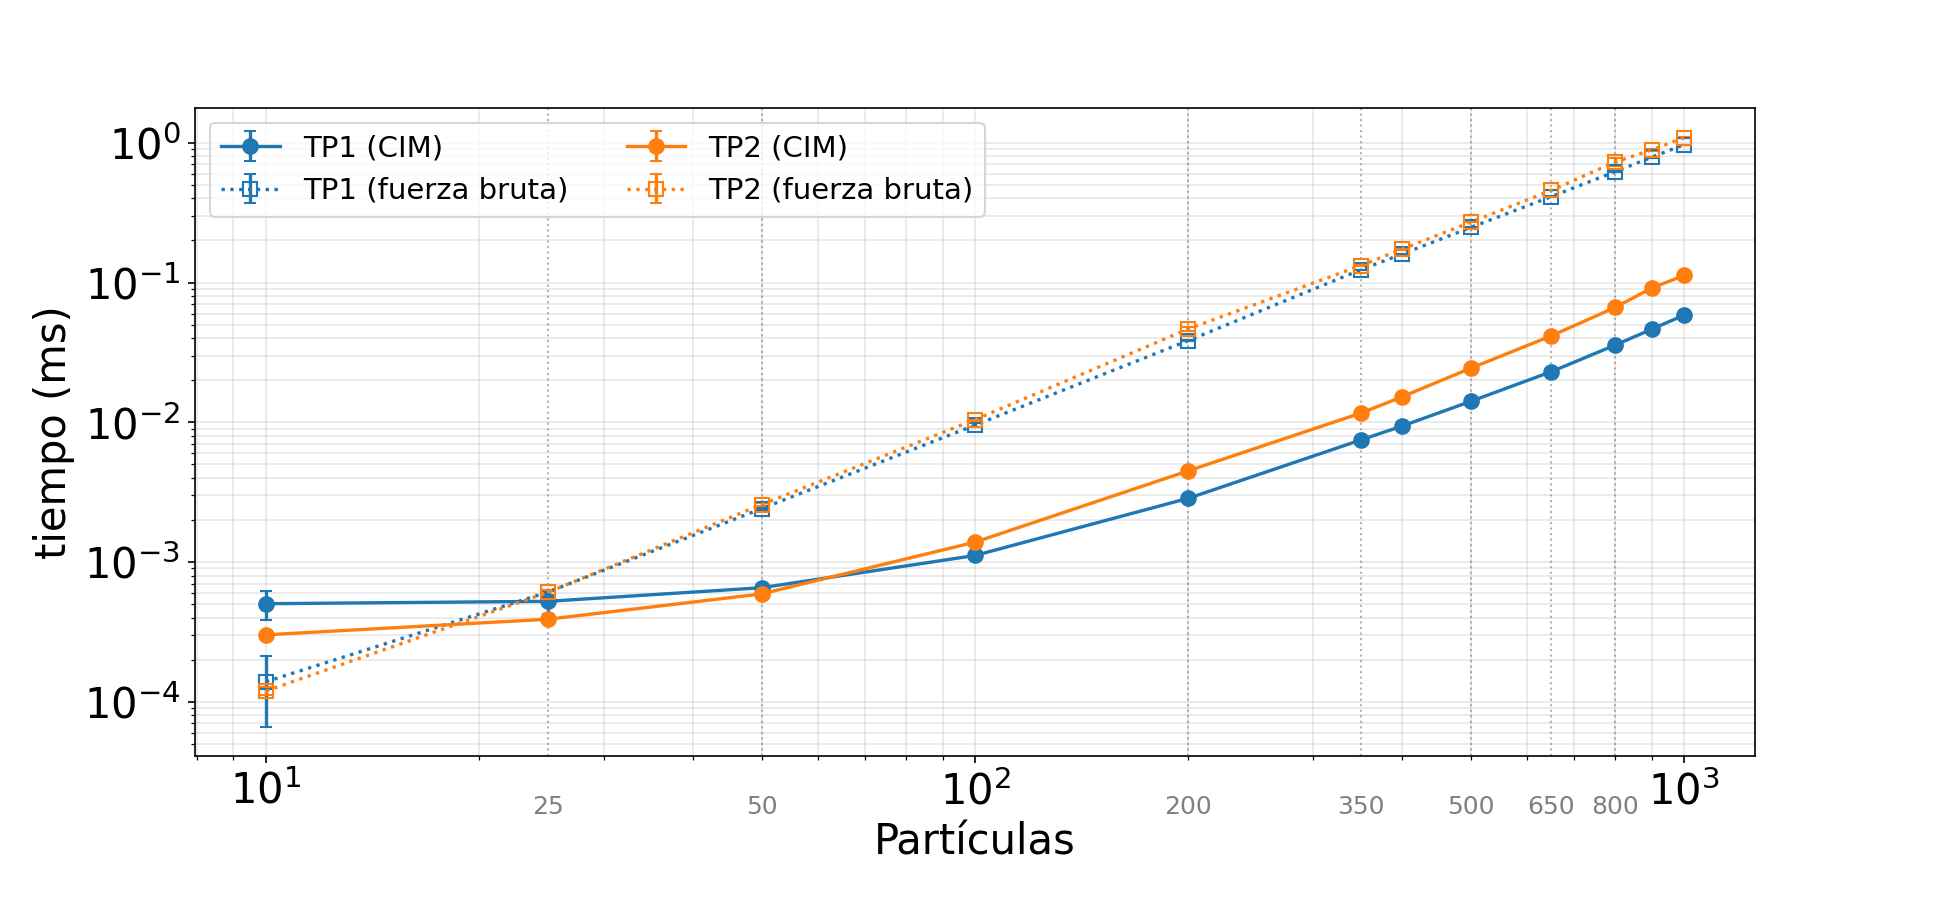
\includegraphics[width=\textwidth,height=0.66\textheight,keepaspectratio]
      {entrega/g/g_cim_vs_tp1.png}
  \end{center}
  \vspace{-0.4em}
  \begin{itemize}
    \footnotesize
    \item Se comparan a igual $N$: el costo del CIM escala con la cantidad de
      particulas, no con la densidad.
  \end{itemize}
\end{frame}

% ============================================================
\section{Conclusiones}
% Frames 56-58
% ============================================================

% --- Frame 56 ---
\seccion{Conclusiones}

% --- Frame 57 ---
\begin{frame}{Conclusiones}
  \begin{enumerate}
    \item % TODO: transicion de fase del modelo estandar segun eta
    \item % TODO: correlacion entre S y va
    \item % TODO: comparacion Estandar vs Votante
    \item % TODO: efecto de la densidad
    \item % TODO: desempeno del CIM
  \end{enumerate}
\end{frame}

% --- Frame 58: Cierre ---
\begin{frame}
  \begin{center}
    \vfill
    {\Huge\bfseries Muchas Gracias}\\[1em]
    {\large Simulacion de Sistemas --- ITBA}\\[0.5em]
    {\large Septiembre 2026}
    \vfill
  \end{center}
\end{frame}

% ============================================================
\end{document}
